% \documentclass[draft,final]{vutinfth} % Remove option 'final' to obtain debug information.
\documentclass[draft, final]{vutinfth} % Remove option 'final' to obtain debug information.

\usepackage{ifxetex}
\ifxetex
    \usepackage{fontspec}
    \defaultfontfeatures{Mapping=tex-text}
    
    %\setsansfont{Fira Sans}
    %\setsansfont{Lato}
    %\setsansfont{Roboto}
    \setsansfont{Source Sans Pro}

    %\setmainfont{Noto Serif}
    \setmainfont{Source Serif Pro}
    
    %\setmonofont{Fira Code}
    \setmonofont{Source Code Pro}
\else
    % Load packages to allow in- and output of non-ASCII characters.
    \usepackage{lmodern}        % Use an extension of the original Computer Modern font to minimize the use of bitmapped letters.
    \usepackage[T1]{fontenc}    % Determines font encoding of the output. Font packages have to be included before this line.
    \usepackage[utf8]{inputenc} % Determines encoding of the input. All input files have to use UTF8 encoding.
\fi

% Extended LaTeX functionality is enables by including packages with \usepackage{...}.
\usepackage{fancyvrb}
\usepackage{listings}
\usepackage{amsmath}    % Extended typesetting of mathematical expression.
\usepackage{amssymb}    % Provides a multitude of mathematical symbols.
\usepackage{mathtools}  % Further extensions of mathematical typesetting.
\usepackage{microtype}  % Small-scale typographic enhancements.
\usepackage[inline]{enumitem} % User control over the layout of lists (itemize, enumerate, description).
\usepackage{multirow}   % Allows table elements to span several rows.
\usepackage{booktabs}   % Improves the typesetting of tables.
\usepackage{subcaption} % Allows the use of subfigures and enables their referencing.
\usepackage[ruled,linesnumbered,algochapter]{algorithm2e} % Enables the writing of pseudo code.
\usepackage[usenames,dvipsnames,table]{xcolor} % Allows the definition and use of colors. This package has to be included before tikz.
\usepackage{nag}       % Issues warnings when best practices in writing LaTeX documents are violated.
\usepackage{todonotes} % Provides tooltip-like todo notes.
\usepackage{hyperref}  % Enables hyperlinking in the electronic document version. This package has to be included second to last.
\usepackage[acronym,toc]{glossaries} % Enables the generation of glossaries and lists of acronyms. This package has to be included last.

\uselanguage{english}
%\renewcommand{\familydefault}{\sfdefault}

%\bibstyle{plain}
%\bibdata{main}

% Define convenience functions to use the author name and the thesis title in the PDF document properties.
\newcommand{\authorname}{Daniel Jonas Otto} % The author name without titles.
\newcommand{\thesistitle}{Virtual Reality as a Catalyst for the Energy Transition} % The title of the thesis. The English version should be used, if it exists.

% Set PDF document properties
\hypersetup{
    pdfpagelayout   = SinglePage,           % How the document is shown in PDF viewers (optional).
    linkbordercolor = {Blue},                 % The color of the borders of boxes around crosslinks (optional).
    pdfauthor       = {\authorname},          % The author's name in the document properties (optional).
    pdftitle        = {\thesistitle},         % The document's title in the document properties (optional).
    pdfsubject      = {Subject},              % The document's subject in the document properties (optional).
    pdfkeywords     = {Photovoltaik, study, VR} % The document's keywords in the document properties (optional).
}

\setpnumwidth{2.5em}        % Avoid overfull hboxes in the table of contents (see memoir manual).
\setsecnumdepth{subsection} % Enumerate subsections.
\nonzeroparskip             % Create space between paragraphs (optional).
\setlength{\parindent}{0pt} % Remove paragraph identation (optional).
% \setlist[itemize]{itemsep=0pt, topsep=0pt, parsep=0pt, partopsep=0pt}
% \OnehalfSpacing
% \sloppy
\hyphenpenalty=800
\tolerance=2000
\emergencystretch=3em

\fvset{
  fontsize=\fontsize{8pt}{10pt}
}
\lstset{basicstyle=\ttfamily\small}

\makeindex      % Use an optional index.
% \makeglossaries % Use an optional glossary.
%\glstocfalse   % Remove the glossaries from the table of contents.

% Set persons with 4 arguments:
%  {title before name}{name}{title after name}{gender}
%  where both titles are optional (i.e. can be given as empty brackets {}).
\setauthor{}{\authorname}{}{male}
\setadvisor{Dipl.-Ing.in Dr.in}{Katharina Krösl}{}{female}

% For bachelor and master theses:
% \setfirstassistant{Pretitle}{Forename Surname}{Posttitle}{male}
% \setsecondassistant{Pretitle}{Forename Surname}{Posttitle}{male}
% \setthirdassistant{Pretitle}{Forename Surname}{Posttitle}{male}

\setregnumber{11811332}
\setdate{10}{5}{2024} % Set date with 3 arguments: {day}{month}{year}.
\settitle{\thesistitle}{Virtual Reality as a Catalyst for the Energy Transition}
% \setsubtitle{Optional Subtitle of the Thesis}{Eine wissenschaftliche Untersuchung des Potenzials von VR-Technologien in der Umweltbildung und -kommunikation}
\setthesis{bachelor}
\setcurriculum{Software and Information Engineering}{Software und Information Engineering}

\begin{document}

\frontmatter % Switches to roman numbering.
% The structure of the thesis has to conform to the guidelines at
%  https://informatics.tuwien.ac.at/study-services

\addtitlepage{english} % English title page.
\addstatementpage

\begin{acknowledgements*}
  I would like to express my gratitude to all those who have provided me with support in the creation of this work. In particular, I would like to thank my partner, Astrid Gaderbauer, for her assistance and understanding throughout this process. I would also like to acknowledge Helwin Prohaska for his invaluable guidance and support in the development of the VR application. Furthermore, I would like to extend my gratitude to my grandparents for their financial support and encouragement. Finally, I would like to express my gratitude to my supervisor, Katharina Krösl, for her extensive guidance and feedback throughout the entirety of this project.

% sandro for helping with the sun simulation formulas
% lukas for the help with implementing the sun calculation in unreal blueprints
\end{acknowledgements*}

% \begin{kurzfassung}
% \todo{Ihr Text hier.}
% \the\baselineskip
% % print fontsize
% \the\fontdimen6\font
% \end{kurzfassung}

\begin{abstract}
This thesis presents the development of a Virtual Reality (VR) application aimed at facilitating the energy transition in Austria. It addresses the widespread perception of the energy transition as overly complex and unachievable, a view that has often led to political inaction and public uncertainty. Through the use of VR technology, this research seeks to demonstrate the necessity and feasibility of transitioning towards renewable energy sources, countering the prevailing skepticism and inertia.

The core of this study lies in creating an immersive VR experience that elucidates the concepts and advantages of the energy transition in an engaging and understandable manner. The application is designed to simplify complex environmental principles, making them accessible and relatable to users. By doing so, it aims to inspire a sense of urgency and possibility regarding the adoption of sustainable energy practices.

This work is grounded in the belief that technological innovation, particularly in the realm of VR, can play a crucial role in environmental advocacy. The goal is to empower individuals with knowledge and perspective, contributing to a more proactive and optimistic approach to environmental challenges in Austria.

The findings and developments from this thesis are expected to offer new pathways in environmental education and communication, highlighting how VR can be a potent tool in promoting understanding and action in the face of environmental challenges. This research aims to stand as a testament to the power of technology in driving societal change, especially in contexts where political leadership may be lacking.
\end{abstract}

\tableofcontents % Starred version, i.e., \tableofcontents*, removes the self-entry.
\mainmatter

\chapter{Introduction}

% One sentence or short paragraph about what the paper is about and a mini-summary of your main results. (1 par) 


% Introducing the important problem you solve, give some (possibly simplified) definitions (1 par)


% Why is this problem important, who has attempted to solve it, which solutions exist so far, why aren‘t they sufficient, why are we left with a dilemma, what are the main obstacles, why would it be useful to fight them. What would be the benefit of a (better) solution. (1/2 page)

...

research questions:
%Wie können die Möglichkeiten von VR genutzt werden, um grundlegendes Verständnis für die Energiewende zu schaffen und die Funktionsweise eines erneuerbaren Energiesystems zu vermitteln?
%1) nutzen von VR generell für verständnis /akzeptanz
1) Can a VR simulation such as the VR application of Energiewende Linz (\textit{KaisergasseVR}) increase understanding/acceptance  and interest for climate-friendly technologies? 

%2) vorteil einer interaktiven sim für photovoltaic
2) Can an interactive photovoltaic use case increase understanding and acceptance of PV solutions?


% Elaboration on single obstacles and how you overcome them.



% Short description of results and their advantage and usefulness in chronological order.


% Some remarks about the nontriviality of the solution 



% Summary of main results in form of a dotlist

contribution:
-) user study and evaluation of \textit{KaisergasseVR}
-) use case designed and implemented (derive from related work) ... as educational tool?
-) user study to evaluate the benefit of a more interactive solution


% Further related work and a sentence about future plans




% Roadmap „This paper is organized as follows... 




This bachelor thesis is dedicated to the development of an innovative Virtual Reality application, which aims to advance the energy transition in Austria. In a context where public opinion and media coverage in Austria often show a certain skepticism towards the energy transition and its challenges, this work aims to bring a positive change and deeper understanding through the use of VR technology.

In Austria, the energy transition is often perceived as complex and controversial in public debate and the news. There is an urgent need to communicate more clearly the benefits and feasibility of this transition. This bachelor thesis aims to positively influence public opinion and promote a deeper understanding of its importance by creating a VR application that conveys the principles and benefits of the energy transition in an interactive and immersive manner.

The work intends to explore the role of VR as a powerful tool in education and communication strategies, to create broader awareness and stronger support for the energy transition among the Austrian population. In doing this, I utilize the latest developments in VR technology and combine them with current environmental issues.

My goal is to make a scientifically founded contribution that considers both the technological aspects and the didactic principles in conveying the challenges and solutions of the energy transition. The work is intended to serve as a basis for future research and applications dealing with the use of VR technology in environmental education and communication.






\chapter{Related Work}

% am besten du machst dir hier als erstes mal ein paar stichworte zur struktur und den main take-aways
% sowas wie:
% VR wird viel in education verwendet (in unterschiedlichen gebieten
% dabei ist besonders wichtig/beneficial/etc: 
% orientierung 
% interaktivität
% collaboration
% ...
% das hab ich jetzt so bissl aus deinem related work raus gelesen. das sind aber eigentlich dinge die gut sind für die argumentation/motivation und daher in die introduction passen. im related work geht es eher darum den state of the art in dem bereich zusammenzufassen. also was gibt es für ähnliche arbeiten? wie unterscheiden sich die? wie sind die besser oder schlechter, etc.

\section{Virtual Reality in Education}

A central aspect in the discussion about the use of Virtual Reality (VR) in education is addressed by Radić-Weissenfeld et al.\cite{hu2017virtual}. This paper offers a profound insight into the diverse applications and the potential of VR as an educational tool in today's era of experience and interactivity.

The authors discuss how VR technologies can revolutionize learning by creating immersive and interactive environments that enable learners to experience complex concepts and systems in a way that is not possible with traditional teaching methods. This approach, aimed at making abstract theories tangible through direct experience, is particularly relevant for the fundamental understanding of the energy transition and renewable energy technologies. The authors emphasize that VR technology offers the possibility to enable learners to experience the impacts of their decisions and actions in a realistic environment. This approach is especially relevant for the energy transition, as it allows learners to understand and experience the effects of their decisions on the environment.

In the context of my work, which aims to improve understanding of the functioning of renewable energy systems through VR, this article provides important insights. The principles of immersion and interactivity described in the article are fundamental pillars for the development of the VR application. In particular, the emphasis on "experience orientation" in the learning process is important for the project, as it is about giving users a deep understanding of the dynamics and impacts of various photovoltaic configurations.

Radić-Weissenfeld et al. also underline the importance of user-centricity in VR learning environments. This aspect is crucial to ensure that our VR application is not only informative but also user-friendly and engaging. By applying these principles, we can create a learning experience that is not only educational but also motivating and inspiring for users.

In conclusion, the article by Radić-Weissenfeld et al. provides an important foundation for our project by demonstrating how VR technology can be effectively used in educational contexts. The insights gained from this directly flow into the design of our VR application, with the goal of creating an intuitive and effective learning experience around the topic of energy transition.
% welche erkenntnisse konkret?

\section{VR Technology in Higher Education: New Perspectives and Applications}

Virtual Reality has established itself as a powerful tool in higher education, especially in the STEM fields (Science, Technology, Engineering, and Mathematics), where VR is predominantly used to make complex and abstract concepts more comprehensible~\cite{ding2022review}. The immersive properties of VR enable students to not only theoretically learn technical and scientific processes but also to grasp them practically and visually, leading to a deeper understanding. This application of VR highlights the technology's potential to make challenging topics more accessible and tangible.

Ding and Li ~\cite{ding2022review} ran a study with ... students to investigate... Their results showed that VR has a significant impact on students' learning outcomes. The use of VR technology in higher education has been observed to improve the absorption and retention of knowledge. VR offers a unique, interactive learning experience that complements and surpasses traditional teaching methods by immersing students directly in the learning environment. This direct, experience-based learning method not only fosters an understanding of complex scientific and technical concepts but also improves long-term retention.

Furthermore, the study emphasizes that VR positively influences students' learning behavior. The incorporation of VR into curricula leads to increased engagement and motivation among students. This technology allows learners to experiment and explore in an interactive and dynamic environment, making learning an active and captivating experience. This not only arouses interest in the subject matter but also enhances problem-solving and critical analysis skills. These changes in student behavior contribute to increasing learning success and fostering a deeper, lasting interest in the topics.

\section{Significant Developments in Educational Virtual Environments}

Mikropoulos and Natsis~\cite{mikropoulos2011educational} provide a comprehensive analysis of research in the field of education-oriented virtual environments (VE) over a ten-year period. This extensive review illuminates the crucial developments and changes that virtual educational environments have undergone in the last decade, thus providing an indispensable basis for understanding the current and future trends in this field.

Mikropoulos and Natsis focus on the diverse applications of VEs in education. They note that VEs are increasingly recognized as effective tools that enrich learning through their immersive and interactive properties in different application areas, from scientific subjects to complex social and cultural topics.

They argue that interactive elements in virtual educational environments can increase learner engagement and motivation, leading to a deeper and more sustainable understanding of the learning content.

Moreover, the authors emphasize the role of VEs in promoting collaborative learning. They demonstrate how virtual environments can support cooperative and collaborative learning, where students can jointly solve tasks and share knowledge, leading to improved understanding and higher retention. This approach is particularly effective as it emphasizes the social aspects of learning, which are often neglected in traditional learning environments.

The researchers also point out the challenges associated with implementing VEs in educational institutions. These challenges include technical limitations, high costs for setting up and maintaining such systems, and the need for adequate training for teachers to effectively use these technologies. They stress the importance of careful planning and support from educational institutions to overcome these challenges.

In conclusion, Mikropoulos and Natsis underscore the potential of VEs as transformative tools in education. They argue that these technologies, when effectively utilized, can revolutionize learning and lead to deeper, more meaningful educational experiences. Their research suggests that VEs could play a key role in shaping future educational strategies, especially in areas that require a high degree of interactivity and engagement.

Given these insights, it is clear that the work of Mikropoulos and Natsis makes an important contribution to the understanding and further development of virtual educational environments. Their research findings provide valuable insights for educational professionals, developers, and researchers working at the intersection of technology and education, forming a solid foundation for future exploration and implementation of VEs in educational contexts.

The insights of Mikropoulos and Natsis are of central importance to my project. Their paper not only offers a deep insight into the historical development and various application areas of virtual educational environments but also serves as a valuable source of inspiration for innovative teaching methods in virtual reality. The importance they place on interactivity in virtual environments is particularly relevant to my project. They provide concrete starting points for designing an interactive and engaging VR learning environment, aiming not just to entertain users but actively involve them in the learning process.

Furthermore, understanding the challenges discussed by Mikropoulos and Natsis -- particularly regarding technical, financial, and pedagogical aspects -- opens the possibility to plan and implement my project realistically and purposefully. This will be crucial for ensuring smooth integration and acceptance of the VR learning application in educational contexts.

In conclusion, the paper forms a sound basis for the development of my VR application. It serves as a compass that highlights both the potentials and pitfalls of using Virtual Reality in education. By taking these insights into account, I can develop an application that is not only technologically advanced but also pedagogically valuable, thus creating an effective and appealing learning experience for users.

\section{Effectiveness and Integration of VR-based Instruction}

The integration of VR-based instruction into traditional teaching methods is a central element of my literature review. This topic is extensively analyzed in the paper "Effectiveness of virtual reality-based instruction on students' learning outcomes in K-12 and higher education"\cite{merchant2014effectiveness}. This meta-analysis explores the effectiveness of VR in various educational contexts and details the specific conditions under which VR can significantly influence learning success. Therefore, it provides valuable insights for the effective use of VR in educational environments. The results are particularly relevant for our project due to the matching age group of the participants and the thematic focus on declarative learning objectives.

Key findings of the paper are:
\begin{itemize}
  \item The results show that VR-based educational environments significantly improve students' learning outcomes. This underscores the potential of VR as an effective tool in education.

  \item The type of learning outcomes, whether knowledge or skill acquisition, influences the effectiveness of VR-based instruction. VR is particularly effective in imparting declarative knowledge. This is relevant for our project as we focus on conveying knowledge about the functioning of photovoltaic systems and the effects of various configurations.

  \item A combination of VR and other teaching methods proves to be particularly effective. This supports an integrated teaching approach where VR is used as a complement to traditional teaching forms. This approach is particularly relevant for our project as we develop the VR application as an addition to workshops in schools.

  \item The nature of feedback and the type of learning tasks are crucial for the effectiveness of VR in an educational context. Detailed explanations are more effective for declarative tasks, while concrete feedback on the correct answer is more effective for procedural tasks. This underlines the importance of tailoring feedback to the type of learning task.

  \item The methodological rigor of study designs influences the observed learning outcomes, with higher methodological rigor leading to stronger evidence of VR's effectiveness. This highlights the importance of careful design of VR-based educational environments.

  \item The results show that VR environments in education increase learner engagement and motivation. Thus, VR serves as a tool to arouse students' interest and actively involve them in the learning process.
\end{itemize}

This paper provides valuable insights for the effective design of VR-based educational environments for my work. It emphasizes the need to carefully design VR applications to ensure they support and complement learning objectives. The insight that a combination of VR and other teaching methods, as well as tailoring feedback to the type of learning task, is crucial for the success of VR in education. These insights will be considered in developing our VR application to ensure an optimal and effective learning experience.

The effectiveness of combining VR with traditional teaching methods highlighted in this paper is already being applied in our project. Our VR application is used in school workshops to make the more abstract content tangible and comprehensible, complementing frontal teaching. This methodological connection helps regain the attention of young people and deepens their understanding of the complex topics of the energy transition. Notably, the potential influence on knowledge retention is enhanced by the interactive and immersive nature of VR.

Based on the findings from the mentioned paper and previous research, I can further develop the VR application by integrating the following elements:

\begin{itemize}
  \item Implementation of interactive feedback systems that allow learners to receive immediate and specific feedback on their actions and decisions within the VR environment. This can be realized, for example, through real-time simulation data and explanatory notes.

  \item Integration of appealing and informative data visualizations that enable users to visualize the immediate effects of their decisions on the environment and energy efficiency. Such visualizations could dynamically display changes in energy amounts, CO2 emissions, or costs depending on the chosen parameters.

  \item Development of additional interactive modules that address specific aspects of the energy transition. These could include simulations that illustrate the effects of different energy systems under selected environmental conditions.

  \item By providing various interaction options within the VR environment, different learning styles can be accommodated. This can be enabled through options for exploratory and structured learning.

  \item Ensuring that the VR application is seamlessly integrated into the preceding and subsequent content of the workshops to create a coherent learning experience. This could be achieved by providing accompanying materials and by coordinating and preparing the content with the teachers.

\end{itemize}

Although the integration of VR into traditional teaching methods is promising, we should review and adjust the effectiveness and relevance of the VR application as necessary. It is important to gather feedback from teachers and students and optimize the application accordingly to ensure that it meets learning objectives and effectively contributes to knowledge transfer.

The insights from the paper and previous studies support the further development of the VR application as an effective tool in education for the energy transition. By specifically adapting and expanding the application, we can further increase learning success and foster lasting interest in the topic. Future research and applications could focus on optimizing the interaction between VR and traditional teaching methods and examining the effects on different learning groups.


\section{VR Applications for Renewable Energy}
% related work
% Works focusing on the use of VR in environmental education and awareness.
% what, how, result, relevance


\chapter{Approach}
\section{Reviewing \textit{KaisergasseVR}}
The association \href{https://www.energiewende-linz.at}{Energiewende Linz} presented their first exhibition at the Ars Electronica Festival in 2022 under the name "PowerPlayGround". This exposition aimed to present multiple interactive stations, each delving into a different aspect of the climate crisis and energy transition. The centerpiece of the exhibit was the recently completed \href{https://www.pilotprojekt-kaisergasse.at/}{Pilotprojekt Kaisergasse Phase 1}, which outlined a comprehensive strategy for making the residential building Kaisergasse 20 Linz more climate-friendly. To visually demonstrate the proposed solutions, the \textit{KaisergasseVR} Virtual Reality application was developed, effectively building on the thematic groundwork established by the preceding stations and strengthening understanding of the solutions.

Participants in \textit{KaisergasseVR} begin their journey in the courtyard of Kaisergasse 20, where they can use a watering can to change dusty dirt into a lush, wild meadow with some trees, visually reducing the surrounding temperature as indicated by a thermometer. The addition of greenery to two nearby commercial building rooftops brings the temperature down to a comfortable 24°C. Accessing these rooftops involves the use of flight capabilities, which are facilitated by the controllers for ascending or descending, with gravity turned off for easy navigation. On the roof of the residential building, semi-transparent solar panel templates became visible. Interacting with these templates via the controllers causes the installation of panel groups, which tints the cables green to indicate electricity generation.
Interacting with these templates via the controllers triggers the installation of panel groups, which turns the cables green to represent electricity generation. Exploring further to the courtyard's garages and parking spots shows four plugs that have been activated by the photovoltaic system. Engaging with these connectors enables the construction of cables to electric car charging stations, visibly discerning which cars are being charged.
Throughout the virtual environment, numerous bubbles invite interaction; clicking on these bubbles reveals 360° photographs that provide a panoramic glimpse into reality, enhancing the experience by bridging the gap between virtual and real-world visuals.

The \textit{KaisergasseVR} simulation aimed to bring the real-world project of installing photovoltaic panels on residential housing to a wider audience. To share the project's experiences, a VR visualization was created for an exhibition at Ars Electronica, assuming that the background information would be provided in a preceding lecture. As a result, the VR functionality was designed to be straightforward.

In the \textit{KaisergasseVR} experience, users can engage in a few key activities: installing groups of PV panels with a few clicks, drawing cables from the house to the charging stations to power them for electric vehicles, and using a "brush" to greenify the courtyard and surrounding flat roofs, which in turn reduces the ambient temperature. The intention behind allowing users to implement these measures themselves within the VR environment is to help them understand and potentially support or initiate similar actions in their own surroundings.

\section{Planning \textit{SolarPowerVR}}
By building the next evolution of \textit{KaisergasseVR} i am able to help bringing the energiewende a step further. My application would  be used at ars electronica and workshops. this should enable us to improve understanding and engagement of many people for climate friendly technologies and actions. 

After some brainstorming it was clear that focusing on one aspect and do it well would wield the best results and are perfect workpiece for my bachelor thesis. Educatiion around the functionality and advantages of photovoltaic systems seemed a very promising endeavor. It is also the aspect where the existing application lacked the most, in my personal opinion.

%I was very excited about helping in making austria more future proof and climate friendly. Developing games was my childhood dream, quite forgotten and labeled unrealistic, this was my big chance in pursuing something meaningful for the future and myself. To build upon the existing application and reuse whats already built, i decided to learn unreal engine from scratch, instead of considering to alternative VR-friendly options like unity and godot. In hindsight it may seem overkill but i completely worked through the tutorials by UnrealSensei and then GameDevTV. This also incorporated in depth the programming of game functionality in C++. This learning stage was extensive and spanned over 4 months.

Subsequently my plan was to use the whole summer to complete the application is best possible condition for the Ars Electronica 2023. Helwin additionally hired the original Developer to fix several bugs in the application and improve the disappointing performance. Working as multiple Developers on the same game is very challenging in Unreal Engine as in any other engine. The game files are binary and impossible to merge different changes through git. To make matters worse the other developer refused to communicate or cooperate. I ended up reapplying my changes over and over when merging the main branch into my new feature. Additionally i volunteered to help realize 2 additional new games which would be showcased in the exhibition. One featured a highly realistic forest fire, the second featured a flood scenario where you are tasked to save the village from the water masses by building dams. I worked around the clock every day to also finish my own application in time. But sadly It just was impossible, regarding my lack of experience and worn mental state.

The Exhibition went smoothly, despite of numerous hardware faults. Following that i had to fully focus on my family and me moving to a new apartment. I was heavily exhausted and was not able to tackle writing the chapter 

%describe the concept:
%1) the whole VR project of Energiewende Linz
%2) new use case (more focus here)

\chapter{Implementation of \textit{SolarPowerVR}}
%implementation details
%describe the technology (UE, plugins)
%structure
%interesting difficult detail (feedback loop)

Vision: The goal is to create an immersive experience, putting the control for the suns position into the users hands and let them observe how the angle affects the power production. To visualize the efficiency throughout the day and also the year, we implement controls to start a simulation window on a specific day of the year and also allow to select this day. The simulation animates the suns position from dawn to dusk, calculating the loss to airmass and the angle efficiency to the PV-Panel and finally showing the resulting generated Power for each Panel and all Panels combined. It is common to design a tailored layout for each roof, allowing to optimize for maximum power output (flat layout) or more balanced output throughout the year (South facing) or more balanced through the day (east-west facing). To enable users to understand the differences, tailored layouts for this specific roof were designed with professional solar layout software. Using the professional results data, we retrofitted this into a modulation of the general formula for determining photovoltaik power output. This allows users to trust in the observed pronciples. This takes into account: Geographical position, Date and Time, Airmass for the resulting sun angle (azimuth and elevation), Angle from Sun to Panel surface.But still there are some limitations, we were not able to consider in this simulation: shadowing, clouds, snow on the panels, varying humidity, transformator and electrical infrastructure loss.

Inline code: \lstinline|This is inline code|.

\begin{Verbatim}
#include <iostream>
int main() {
    std::cout << "Hello, world!";
    return 0;
}
\end{Verbatim}

% The choice to focus on photovoltaics was driven by the conviction that the mechanics of photovoltaic systems, with their multifaceted factors, are best experienced intuitively through experimentation and observation within a VR environment. This immersive approach aimed to demystify the complexities associated with the energy transition, fostering a broader acceptance and initiative in this critical area.

\chapter{Evaluation}
This chapter outlines the evaluation process of the two virtual reality (VR) applications \textit{KaisergasseVR} and \textit{SolarPowerVR}. The primary objective was to assess whether \textit{SolarPowerVR} could contribute more than \textit{KaisergasseVR} to participants' understanding and engagement with climate-friendly technologies, with a particular focus on photovoltaic solutions. The user studies were conducted following participants' engagement with the respective VR application. Participation in this post-experience survey was optional.

The initial evaluation began with the \textit{KaisergasseVR} application, which served as a baseline. This user study was conducted to assess the effectiveness of a VR application in raising awareness and influencing attitudes towards climate-positive actions within an urban environment. We aimed to determine the application's effectiveness in conveying the utility of climate-friendly actions and to identify areas needing enhancement.

Building upon the established baseline and feedback, \textit{SolarPowerVR} was designed to incorporate more interactive elements and observational opportunities to engage users deeply. While continuing to target the primary goals of further increasing understanding and interest in PV solutions, it also aimed to additionally impart factual knowledge through observation, such as the optimal orientation of photovoltaic panels. This secondary goal explores whether deeper engagement and interactivity can contribute to more comprehensive learning outcomes.

\section{User study on \textit{KaisergasseVR}}
The evaluation took place in a large hall within the JKU building during the JKU Games 2023S.  We provided an open booth that was available from 14:00 to 01:00, with at least two helpers present at all times to assist participants and monitor station activities.

The setup included three VR stations, each offering a different experience:
\begin{itemize}
    \item A PCVR station using a Meta Quest 2, exclusive to \textit{KaisergasseVR}.
    \item A PCVR station equipped with an HP Reverb G2 headset offering a choice of \textit{KaisergasseVR}, \hyperlink{https://store.steampowered.com/app/517160/Richies_Plank_Experience/}{Richie's Plank Experience} and \hyperlink{https://store.steampowered.com/app/620980/Beat_Saber/}{Beat Saber}.
   \item A standalone Meta Quest 2 station with Beat Saber.
\end{itemize}

\subsection{Study Protocol}
 Participants were invited to experience the VR simulation, which encouraged a dynamic interaction scenario. Before starting the VR experience, participants were given detailed instructions about the VR equipment and the goals of the simulation as the VR application itself contained no instructions. This approach was necessary to ensure that participants could effectively navigate the VR environment and understand the solutions presented. Those who experienced \textit{KaisergasseVR} were then invited to fill out the user study form.

\subsection{Questionnaire Design}
The questionnaire covered a wide range of topics, including demographic information and detailed questions about climate change awareness, as well as specific feedback on the VR experience. Structured as follows, it began with an informed consent declaration followed by basic demographic questions (age, gender). Subsequent sections addressed participants' attitudes towards climate change, their personal engagement with eco-friendly practices, and their familiarity with VR technologies. The survey contained both Likert-scale questions (from 1: strongly disagree to 5: strongly agree) and open-ended questions. Specific questions related to the VR experience included:
\begin{itemize}
    \item Evaluation of ease of navigation and realism within the VR environment.
    \item Assessment of the educational effectiveness of the VR simulation concerning urban thermal conditions and photovoltaic systems.
    \item Personal inclination towards real-world application of the observed technologies post-simulation.
    \item Open-ended questions for detailed feedback and suggestions for improvements.
\end{itemize}

Although the questionnaire turned out to be more extensive than necessary for statistical analysis, it provided valuable insights into the participants' perceptions and highlighted interesting findings for potential exploratory analysis.

\subsection{Data Collection and Analysis Methods}
Data was collected through Google Forms, allowing for seamless distribution and accessibility via QR codes that participants could scan with their mobile devices or access through a laptop provided at the site. The responses were later exported to a CSV file and analyzed using Python.

\subsection{Participants}
The study included 14 participants, with an age distribution as follows: under 20 (2), 20-29 (11), and 30-39 (1). The gender breakdown included nine males and five females. Participants' backgrounds and attitudes were assessed using a Likert scale.

Participants reported moderate familiarity with VR technologies (mean: 3.29, SD: 1.33), indicating varied experience levels. The participants demonstrated a high level of agreement on the significance of climate change (mean: 4.07, SD: 0.59). They also exhibited a willingness to engage in energy transition activities (mean: 4.21, SD: 0.67), indicating a positive inclination towards environmental action. Furthermore, they expressed a strong belief in the impact of climate change on urban quality of life (mean: 4.86, SD: 0.35). There was a moderate level of interest in eco-electricity (mean: 4.00, SD: 1.25). These responses are visually summarized in \figurename~\ref{fig:participants_kaisergasse}.

\begin{figure}[h]
    \centering
    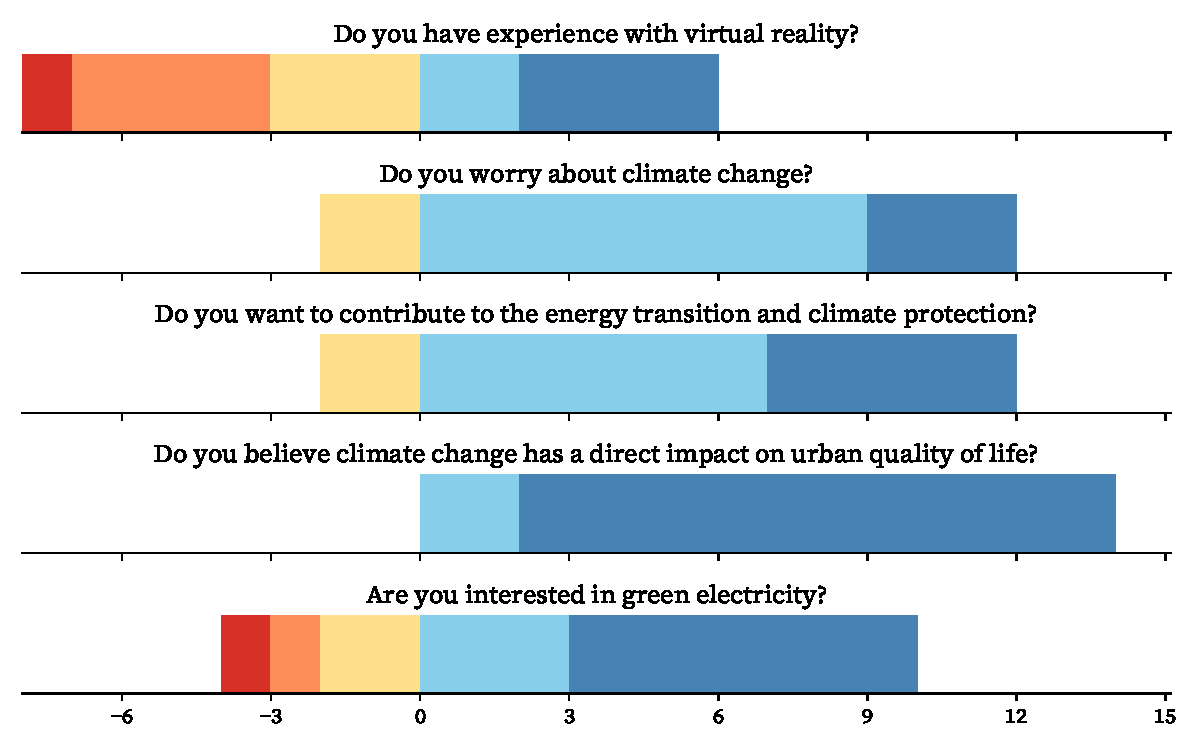
\includegraphics[width=\textwidth]{graphics/participants-kaisergasse.pdf}
    \caption{Stacked bar chart of participant responses to personal questions in the \textit{KaisergasseVR} study. The chart displays answers to questions assessing participants' experience with virtual reality, concerns about climate change, willingness to contribute to energy transition and climate protection, perceptions of climate change's impact on urban quality of life, and interest in green electricity.}
    \label{fig:participants_kaisergasse}
\end{figure}

\section{User study on \textit{SolarPowerVR}}
The user study on \textit{SolarPowerVR} was conducted during the ``VR-Day'' event at HLW Steyr. This event was attended by students from one class of HLW Steyr and lasted three hours, from 13:00 to 16:00. The event began with a detailed presentation on the ongoing challenges and achievements in energy transition, including a highlight of our exhibition at Ars Electronica 2023. This served to set the context for the importance of renewable energy solutions, specifically photovoltaic systems. Following the presentation, students had the opportunity to experience \textit{SolarPowerVR} and various VR games. The feedback was overwhelmingly positive.

The setup included four PC-VR stations, each offering a different experience:
\begin{itemize}
    \item Two stations dedicated to \textit{SolarPowerVR}, one equipped with a Meta Quest 3 and the other with a Meta Quest 2.
    \item Interactive experiences with \hyperlink{https://store.steampowered.com/app/517160/Richies_Plank_Experience/}{Richie's Plank Experience} and \hyperlink{https://store.steampowered.com/app/620980/Beat_Saber/}{Beat Saber}, both running on Meta Quest 2.
\end{itemize}

This event marked the first public access to the \textit{SolarPowerVR} app, providing an excellent opportunity for gathering study data and valuable feedback. Participation in trying out VR apps was voluntary, as was completing the post-experience survey. A total of 10 students filled out the form at this event.

Additional sessions were later held at HTL Linz (n=5) and my office (n=3) to collect more data and increase the robustness of our dataset.

\subsection{Study Protocol}
Participants were individually invited and given a presentation on the interactive elements of \textit{SolarPowerVR} individually. The instructional session covered navigation, photovoltaic layout selection, adjusting the month for simulation, starting/stopping the simulation run, and data interpretation within the VR environment. This upfront guidance was crucial as participants were then expected to explore the application independently.

The instructional session followed a prepared schema with a presentation lasting approximately 3 minutes. This ensured users would have an easy time navigating through the app; however, I remained available to assist if needed. To refine this protocol, it was tested once with my girlfriend prior to the main event. Based on this test, I added an in-game button schema for better user guidance.

After familiarizing themselves with the setup, participants put on their VR headsets and freely explored the simulation. Upon completion, they were invited to provide their insights and feedback through our user study form.

\subsection{Questionnaire Design}
The questionnaire for this study aimed to assess participants' perceptions of climate change and their experience of the VR simulation. It contained Likert-scale questions (from 1: strongly disagree to 5: strongly agree), multiple-choice questions, and open-ended questions structured around key components:
\begin{itemize}
\item Initial questions collected demographic data and assessed participants' familiarity with VR technology and their concerns about climate change.
\item Participants responded to questions about usability and realism of the VR simulation, its effectiveness in conveying benefits and applications of photovoltaic systems, and their likelihood of engaging in climate-positive actions following their experience.
\item Specific questions tested understanding of optimal orientation of photovoltaic panels for different seasons, directly measuring educational outcomes from the VR experience.
\item Open-ended questions invited comments on what participants liked most and least about their experience as well as suggestions for improvement.
\end{itemize}

The decision to use a 5-point Likert scale was made to ensure comparability with the previous study on \textit{KaisergasseVR}. While it may not capture all nuances, it provides a rough picture that is still valuable for analysis.

\subsection{Data Collection and Analysis}
Data was collected through Google Forms for seamless distribution via QR codes that participants could scan with their mobile devices. Responses were later exported to CSV files for analysis using Python.

\subsection{Participants}
The participant cohort consisted of 18 individuals, primarily young students (mean age: 19.11 years: SD: 5.96). Their familiarity with VR technology was modest (mean: 2.72, SD: 1.28), providing a unique perspective on the educational potential of immersive VR applications such as \textit{SolarPowerVR}. Participants expressed moderate concern about climate change (mean: 3.50, SD: 1.01) and a commendable willingness to engage in activities related to energy transition and climate protection (mean: 3.83, SD: 0.69). The perceived impact of climate change on urban quality of life was particularly high (mean: 4.28, SD: 0.93), while interest in using green electricity was more variable (mean: 3.33, SD: 0.75). These responses are summarized visually in \figurename~\ref{fig:participants_solarpowervr}.

\begin{figure}[h]
    \centering
    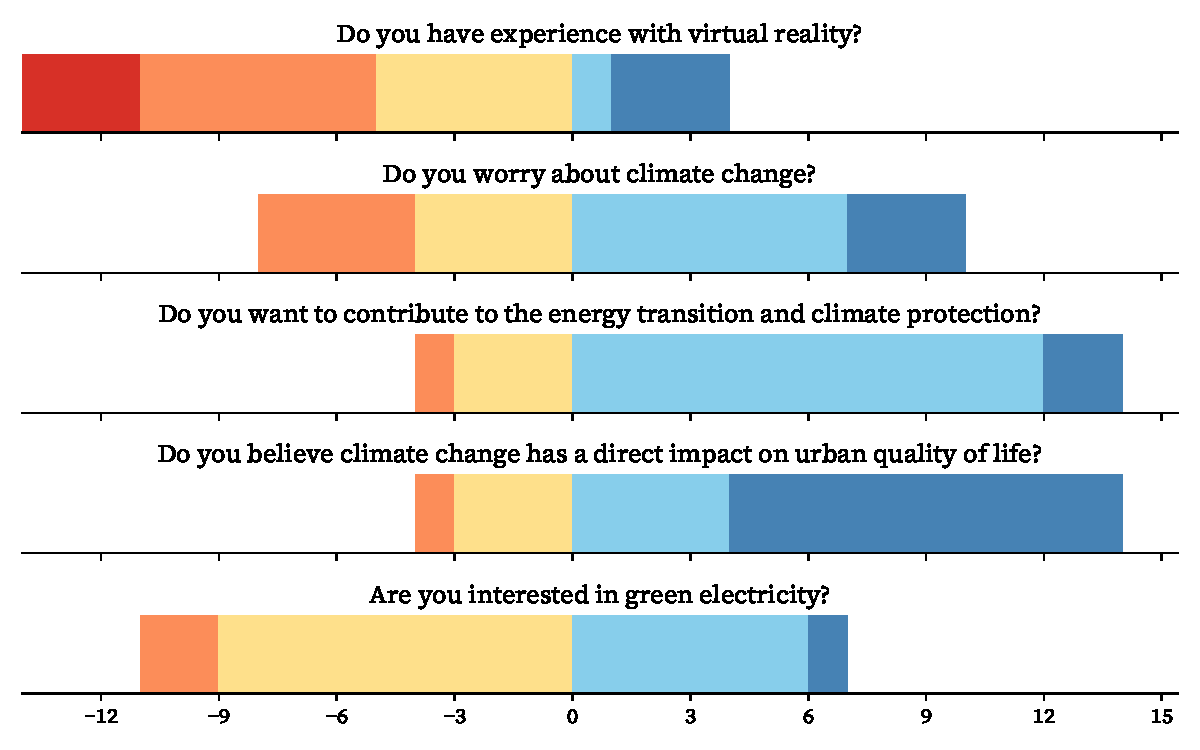
\includegraphics[width=\textwidth]{graphics/participants-solarpowervr.pdf}
    \caption[Participant Responses Summary]{Stacked bar graph showing participants' responses to personal virtual reality experiences, concerns about climate change, engagement in energy transition and climate action, perceived impact on urban quality of life, and interest in green electricity.}
    \label{fig:participants_solarpowervr}
\end{figure}

\chapter{Results}
This chapter presents the findings of two empirical studies designed to assess the efficacy of virtual reality (VR) applications as educational instruments for enhancing comprehension of sustainable technologies, with a particular emphasis on photovoltaic (PV) systems. The initial study on \textit{KaisergasseVR} serves as a baseline for evaluating the impact of immersive VR experiences on environmental education. Subsequently, the \textit{SolarPowerVR} study builds upon this foundation by focusing on the educational outcomes related to solar energy.

The methodologies employed in these studies were intentionally pragmatic, aiming to balance rigorous scientific inquiry with the flexibility necessary to adapt to the evolving nature of VR technology. This approach allowed for the collection of valuable data while acknowledging the exploratory phase of integrating VR into educational settings.

The results of these investigations indicate that VR has the potential to be a valuable tool in the educational domain. The findings demonstrate that VR can enhance cognitive understanding of complex environmental systems, such as PV installations, and foster increased awareness of sustainable practices. Furthermore, the studies suggest that VR-based educational tools can be an effective motivator for individuals to engage in pro-environmental behaviors.

In pursuit of academic integrity and to facilitate future research endeavors, the complete statistical analyses, along with anonymized datasets, have been made publicly accessible. Those interested in examining and verifying the study's outcomes are invited to visit the following repository, where the Jupyter notebook containing all statistical procedures and data is hosted.
\begin{center}
\url{https://github.com/Nelathan/SolarPowerVR-Study}
\end{center}

The subsequent sections will present a detailed examination of the results from both studies, offering insights into the effects of VR on learning about PV systems and discussing the broader implications for environmental education.

\section{User Feedback on \textit{KaisergasseVR}}
The evaluation of the \textit{KaisergasseVR} application demonstrated generally positive user interactions with the virtual environment, as reflected by the score for ease of navigation (mean: 4.00, SD: 0.85). This suggests that the majority of participants found the VR environment user-friendly and intuitive.
The realism of the VR simulation was rated moderately high (mean: 3.64, SD: 0.89), indicating a good level of immersion but also room for improvement.
The participants demonstrated a relatively positive response to the idea of installing a PV system (mean: 3.57, SD: 1.05). This indicates a slight inclination towards actual implementation, inspired by the VR experience.
The VR simulation had a moderate impact on inspiring participants to engage in climate action (mean: 3.14, SD: 1.36). Although this indicates a certain degree of motivation towards environmental involvement, the considerable standard deviation suggests that the responses of the participants were not uniform.

\begin{figure}[h]
    \centering
    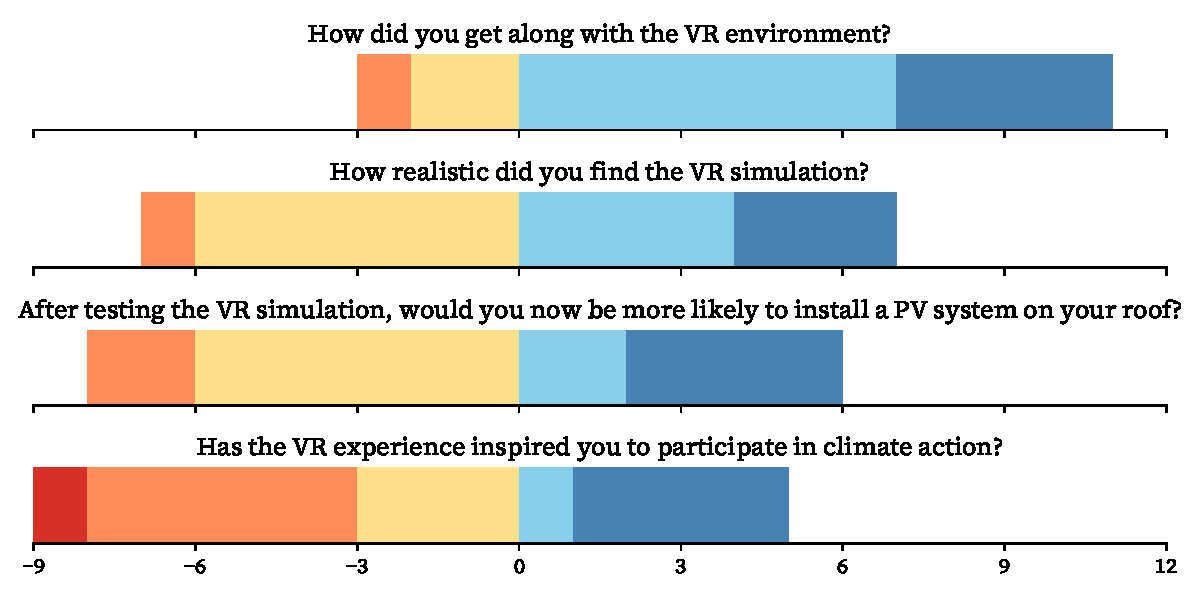
\includegraphics[width=\textwidth]{graphics/feedback-kaisergasse.pdf}
    \caption{Stacked bar chart illustrating the distribution of participant responses to several feedback questions in the \textit{KaisergasseVR} study, including ease of navigation, realism of the simulation, likelihood of installing a PV system, and motivation to engage in climate action.}
    \label{fig:feedback-kaisergasse}
\end{figure}

The participants offered a wealth of insights into the strengths and areas for improvement of the VR application. A synthesis of the responses to the open-ended questions is provided below. 

% Die einfache durchführung und verschiedenen Optionen in Operationen
% war ganz nett
% echten 3d aufnahmen
% Der Vergleich von Simulation und echter Welt
% Thematik
% Vergleich mit der realen Aufnahmen
% Begrünen, weil die Auswirkungen am Greifbarsten sichtbar ist.
% eine sehr bekannte Umgebung (in meinem Fall die Nachbarschaft). Dass reale Aufnahmen von der Drohne eingebaut wurden. Die Variation der Wiese ist echt gut gelungen. Die Gestaltung des Hofes, die Aufgaben und die Bilder der Umgebung

\textbf{Positive Aspects:}
\begin{itemize}
    \item Participants appreciated the \textbf{simplicity and variety of operations} within the VR environment, highlighting the ease of interaction and the range of options available.
    \item The integration of \textbf{360° photographs} was well received and provided a compelling comparison between the virtual simulation and real environments. % not photogrammetry
    \item The \textbf{theme and relevance} of the content resonated with users, emphasizing the importance and appeal of climate-positive actions.
    \item The \textbf{tangible visibility of environmental impact}, particularly through activities such as greening, significantly increased user engagement.
    \item The \textbf{familiarity} of the environment and the quality of the visual elements, such as the variation in the grass and the design of the courtyard, were highlighted as immersive aspects of the experience.
\end{itemize}
% TODO: add citation of real user answer: ... with one user even pointing out that

% Nicht gut gefallen hat:
% Die Framerate und manchmaliges stocken für zu schwindelgefühle
% Photovoltaik und Stromleitungen legen hat nocht wirklich was gezeigt. Klar, Akku wurde gefüllt. Aber was sind die Auswirkungen? Wie schnell wurde wie viel Energie erzeugt? (Z.B. Kilometer, die man mit dem Auto dann im Schnitt fahren kann)
% texturen 
% Schwindelanfälle beim Fliegen
% im Vergleich zu professionelleren Spielen wird einem relativ leicht übel
% Die Orientierung ist noch ein bisschen gewöhnungsbedürftig, weil die Ansicht "fixed" ist, wenn man sich zur Seite dreht und kenie 360° Drehung möglich ist. 
% die PV Anlage hatte wenig offensichtlichen Nutzen, bei Bewegungen wird einem schwindlig
% Motion Sickness durch das Fliegen

% Verbesserungsvorschläge:
% Untersuchung und testung woran die aussetzer in der Bewegung liegen könnte, wäre noch gut
% bessere texturen
% weniger Ruckler
% Umsehen ruckelt sehr
% Auf der Blumenwiese fehlen noch die summenden Bienen :)
% Je nach dem wie aufwändig und ressourcenabhängig es ist: Deko wäre ganz toll und macht die Umgbung um vieles freundlicher. (Der Raum mit der Erde ist z.B. sehr lieblos gestaltet und ist ein bisschen gruselig.) -vl. mehr Leben integrieren? (Andere Menschen die dann zum E-Auto gehen, laufende Hunde, Vögel, bewegte Schatten von vorbeiziehenden Wolken)
% Der Raum mit der Erde bräuchte eine Beschreibung um was es da geht (sofern er einen Sinn hat). Ich hab mich recht verloren gefühlt. Eine weitere Idee wäre, dass man die eigenen Hände in der VR sehen kann - würde der Orientierung mit den Werkzeugen helfen, wenn diese nicht so herumschweben, sondern von Händen gehalten werden. 
% Die Drehfunktion sollte nicht ein plötzlicher Sprung sein

\textbf{Areas for Improvement and Enhancement Suggestions:}
\begin{itemize}
    \item \textbf{Frame rate and navigation:} Users experienced discomfort due to frame rate issues and occasional stuttering, particularly during flight sequences. Improving the smoothness of movement and introducing a more intuitive rotation mechanism could reduce motion sickness and improve navigation within the VR environment.

    \item \textbf{Utility and Impact Visibility:} The application's demonstration of certain features, particularly the photovoltaic installations, was considered inadequate. Users suggested making the results of actions more visible and understandable, for example by showing the real-world impact of energy production in terms of tangible benefits (e.g. kilometres driven by an electric vehicle powered by the energy produced).

    \item \textbf{Environmental detailing:} The quality of the environmental elements was identified as an area for improvement. Suggestions included enriching the VR environment with more detailed textures, dynamic elements such as animals and people, and decorations to create a more immersive and vibrant environment.

    \item \textbf{Innovative Features:} The proposed feature to simulate energy production based on solar panel orientation received positive feedback. Users liked the idea and recommended the use of visual cues to indicate energy output levels and the inclusion of environmental variables to add depth to the educational content of the VR experience.

    \item \textbf{Frame rate and navigation:} Our study revealed that users experienced discomfort due to frame rate issues and occasional stuttering, particularly during flight sequences. One common concern was that \textit{``Umsehen ruckelt sehr''}, which suggests that improving the smoothness of movement and introducing a more intuitive rotation mechanism could reduce motion sickness and improve navigation within the VR environment.

    \item \textbf{Utility and Impact Visibility:} Our results showed that the application's demonstration of certain features, particularly the photovoltaic installations, was considered inadequate. Participants noted that the experience lacked a sense of accomplishment, with one user commenting that \textit{``Auf der Blumenwiese fehlen noch die summenden Bienen''}. This suggests that making the results of actions more visible and understandable, for example by showing the real-world impact of energy production in terms of tangible benefits (e.g. kilometres driven by an electric vehicle powered by the energy produced), could enhance the user experience.

    \item \textbf{Environmental detailing:} Our study revealed that the quality of the environmental elements was identified as an area for improvement. Participants recommended enriching the VR environment with more detailed textures, dynamic elements such as animals and people, and decorations to create a more immersive and vibrant environment. For example, one user suggested that \textit{``Deko wäre ganz toll und macht die Umgebung um vieles freundlicher''}.

    \item \textbf{Innovative Features:} Our findings indicate that the proposed feature to simulate energy production based on solar panel orientation received positive feedback. Participants liked the idea and recommended the use of visual cues to indicate energy output levels and the inclusion of environmental variables to add depth to the educational content of the VR experience. For instance, one user pointed out that \textit{``die eigenen Hände in VR sehen, das würde der Orientierung mit den Werkzeugen helfen''}.
\end{itemize}

This user feedback has had a significant impact on the design and development of the \textit{SolarPowerVR} application, addressing previous shortcomings. The new application provides a user-centric experience by focusing on \textbf{improving user comfort}, \textbf{enriching the visual and interactive quality} of the environment, and \textbf{effectively communicating the impact of climate positive actions}.

\section{User Feedback on \textit{SolarPowerVR}}
Participants' interactions within the VR environment were very positive in terms of ease of navigation (mean: 4.39, SD: 0.59).
The realism of the VR simulation received a moderately high rating (mean: 3.78, SD: 0.92), suggesting a convincing yet variable experience across users.
Concerning the potential for action, the simulation influenced participants' willingness to install photovoltaic (PV) systems on their roofs (mean: 3.33, SD: 1.00), indicating a cautious yet positive inclination towards real-world application.
Additionally, the VR experience played a role in inspiring climate action, although to a lesser extent (mean: 3.00, SD: 0.75).
% use same structure as in 6.1

\begin{figure}[h]
    \centering
    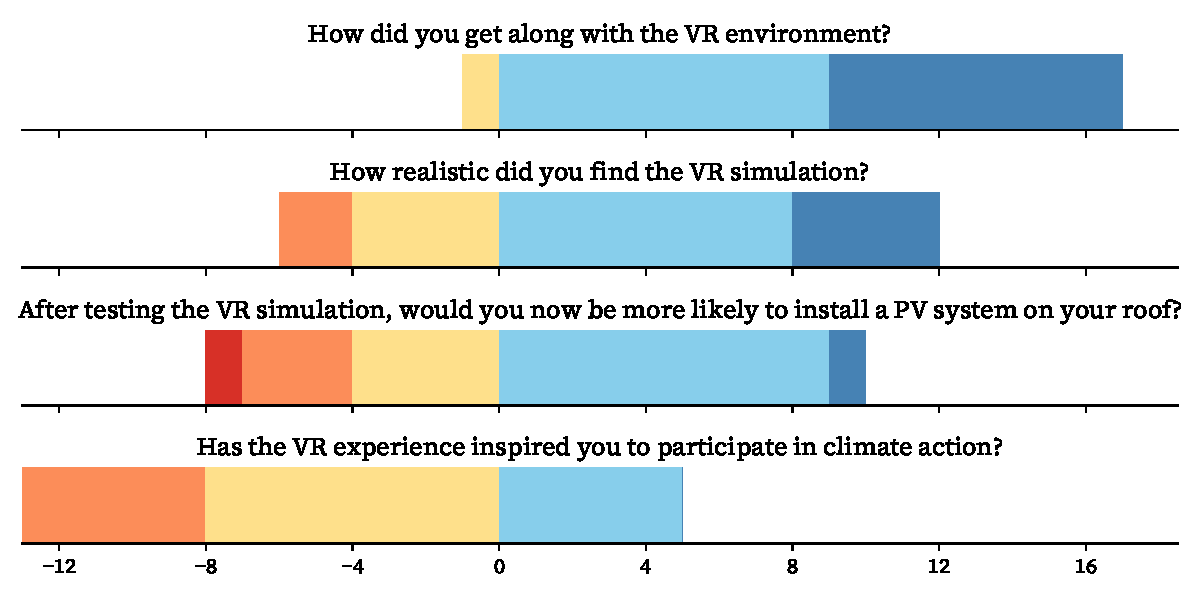
\includegraphics[width=\textwidth]{graphics/feedback-solarpowervr.pdf}
    \caption{Stacked bar chart illustrating the distribution of participant responses to feedback questions in the \textit{SolarPowerVR} study, including ease of navigation, realism of the simulation, likelihood of installing a PV system, and motivation to engage in climate action.}
    \label{fig:feedback-solarpowervr}
\end{figure}

The participants expressed a variety of aspects that they enjoyed about the VR experience. Many appreciated the ability to interactively adjust settings such as the month and time of day and how it affected energy calculations. One participant noted, "I liked that you could adjust so many settings (months, time, ...)" and another mentioned, "The realistic representation of how different setups would look on a rooftop was particularly engaging." The realistic environment and features like the data displayed on the roof and the hands-on experience of building and navigating within the virtual space were frequently praised. Users expressed appreciation for the ability to observe the number of panels required to generate specific amounts of energy. The aesthetic quality of the simulation and its AI assistant were identified as positive features, which enhanced the overall immersive experience.

However, certain aspects of the VR experience were less satisfactory. Some users reported issues with the AI assistant not functioning properly, as one participant noted, "The AI assistant didn't work unfortunately." Additionally, a few found the activities within the virtual environment (VE) limited and expressed a desire for a bird's-eye view of the roof, stating, "You couldn't see the roof from a bird's-eye view." Suggestions for improving the VR experience included enhancements to the AI assistant to make it more reliable and interactive. It was recommended that the nighttime settings be brightened to improve visibility, that the virtual environments be expanded to include various places such as cities, parks, countries, or forests, and that additional options be integrated, such as wind turbines. Furthermore, participants suggested that more activities be included within the VR environment, that step-by-step instructions on tasks be provided, and that interaction opportunities with the AI character be increased. It was also proposed that offering more panel types and configurations could enrich the educational aspect of the simulation.

\section{Impact of VR on understanding and interest in climate-friendly technologies}

To answer research question 1 (\textit{Q1: Can a VR simulation such as \textit{KaisergasseVR} increase understanding of and interest in climate-friendly technologies?}) we tested the following two hypotheses.

\textbf{Hypothesis 1: VR applications such as \textit{KaisergasseVR} increase participants' understanding of climate-friendly technologies.} 

We analyze participants' responses to post-experience question items designed to evaluate their understanding. The questions, rated on a scale of 1 to 5 (with 5 indicating a high level of understanding and 1 indicating a low level), include
\begin{itemize}
    \item Did the VR experience help you understand the actions that can be taken to improve urban thermal conditions?
    \item Did the VR experience help you understand the benefits of these actions?
\end{itemize}
We expected that scores above the mean of 3 would indicate a successful increase in understanding due to the VR experience.

\begin{figure}[h]
    \centering
    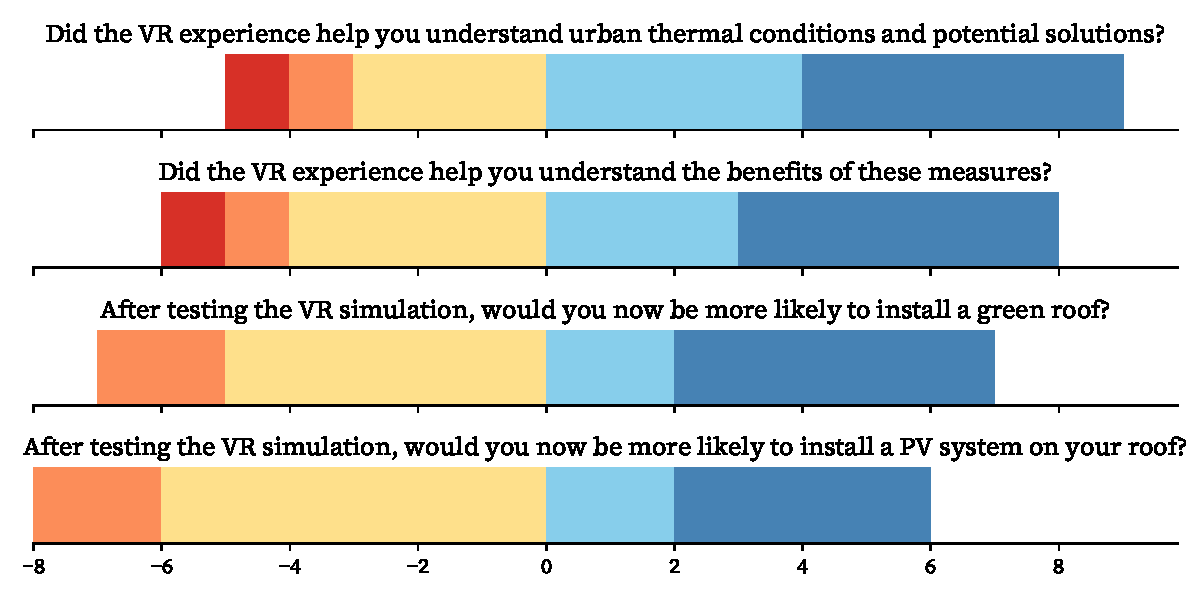
\includegraphics[width=\textwidth]{graphics/research-1.pdf}
    \caption{Stacked bar chart of participant responses to the question on understanding actions to improve urban thermal conditions and the benefits of these actions}
    \label{fig:research-1}
\end{figure}

The Shapiro-Wilk test was first used to check the normality of the response distribution, giving values of 0.865 (p=0.036) and 0.874 (p=0.048) for the two questions respectively. These results indicated a deviation from the normal distribution, necessitating the use of the non-parametric Wilcoxon test, which is appropriate for small non-normally distributed samples.

The Wilcoxon test produced a statistic of 54.5 with a p-value of 0.02466 for the first question and a statistic of 45.0 with a p-value of 0.03301 for the second question. These initial p-values suggested a statistically significant effect (when compared to the standard alpha value of $\alpha = 0.5$ of the VR experience on comprehension. However, after applying the Bonferroni correction to account for multiple testing (4 tests for this research question), the results were not statistically insignificant when compared to the adjusted alpha-values ($\alpha = ?$), leading to the retention of the null hypothesis for both question items.
%add alpha
In conclusion, while the initial analysis suggested a potential impact of the \textit{KaisergasseVR} on improving participants' understanding of climate-friendly technologies, the application of the Bonferroni correction revealed that these effects did not meet the threshold for statistical significance. This indicates that, based on this strict statistical criterion, the VR simulation did not significantly improve participants' understanding as originally hypothesized.

\textbf{Hypothesis 2: VR applications such as \textit{KaisergasseVR} stimulate increased interest in adopting climate-friendly technologies.} 

Participants' responses to post-experience questions will assess their interest in adopting climate-friendly actions. Responses will be rated on a scale of 1 to 5, with 5 indicating high likelihood and 1 indicating low likelihood:
\begin{itemize}
    \item Would you be more likely to install a green roof after testing the VR simulation?
    \item Would you be more likely to install a PV system on your roof after testing the VR simulation?
\end{itemize}
It is expected that scores above the median of three will indicate an increased interest in implementing green technologies, confirming the impact of \textit{KaisergasseVR}.

The Wilcoxon test was chosen due to the non-normal distribution of participants' responses, as indicated by the Shapiro-Wilk statistic (0.842, p=0.017 for green roofs and 0.849, p=0.022 for PV systems). Our null hypotheses were that the VR simulation had no significant effect on participants' willingness to adopt green roofs or PV systems in the real world.

The mean scores (3.71 for green roofs and 3.57 for PV systems) indicated a reasonable level of interest. However, the results of the Wilcoxon test (statistics of 40.0 for green roofs and 31.0 for PV systems, with p-values of 0.01658 and 0.03097 respectively) initially suggested that the VR experience might have a positive effect. After applying the Bonferroni correction (to account for multiple comparisons), these effects were deemed statistically insignificant, leading to the retention of the null hypotheses that the VR simulation had no significant effect on participants' willingness to adopt green roofs or PV systems.

%\section{Can an interactive photovoltaic use case increase understanding of and interest in PV solutions?}
\section{The Impact of Interaction}

To answer.....

\textbf{Hypothesis 3: Interactive engagement with a photovoltaic use case in the VR application significantly increases both understanding of and interest in PV solutions.} 

To evaluate this hypothesis, we analyse responses to two key questions included in both study questionnaires, focusing on the role of the VR experience in deepening understanding of PV systems. Responses were collected on a scale of 1 to 5, with 5 being "very helpful" and 1 being "not helpful at all".


\begin{figure}[h]
    \centering
    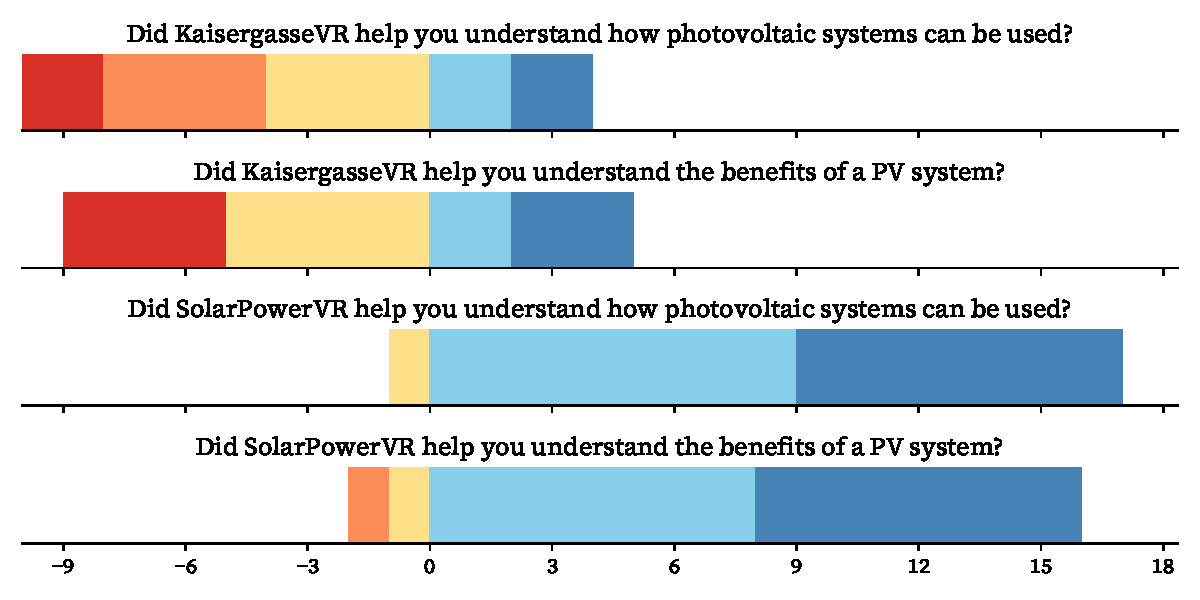
\includegraphics[width=\textwidth]{graphics/research-2.pdf}
    \caption{Stacked bar chart of participant responses on understanding the use and benefits of photovoltaic systems in each application.}
    \label{fig:research-2}
\end{figure}

%TODO: use n, mean, sd in description

The final survey data was found to be non-normally distributed for both the understanding of PV system utilization (p=0.000) and the benefits of PV systems (p=0.029), as indicated by the Shapiro-Wilk test. Therefore, the one-sided Mann-Whitney U test was used.

The results showed a significant effect, with the null hypothesis being rejected for both aspects of understanding a PV system's usage (U=211, p=0.000419) and benefits (U=190, p=0.005654). The study shows that the use of interactive VR had a significantly greater positive impact on participants' understanding and interest in PV solutions than .... . This evidence strongly supports the effectiveness of interactive VR simulations in improving understanding and stimulating interest in photovoltaic technologies.

\section{How does an interactive VR simulation increase factual knowledge regarding the optimal orientation of photovoltaic panels?}

This research question focuses on the ability of the VR simulation to increase factual knowledge related to the strategic placement of photovoltaic panels to optimize electricity production at different times of the year.

\textbf{Hypothesis 4: Experiencing \textit{SolarPowerVR} can increase factual knowledge about the optimal orientation of photovoltaic panels for electricity production.} 

\begin{figure}[h]
    \centering
    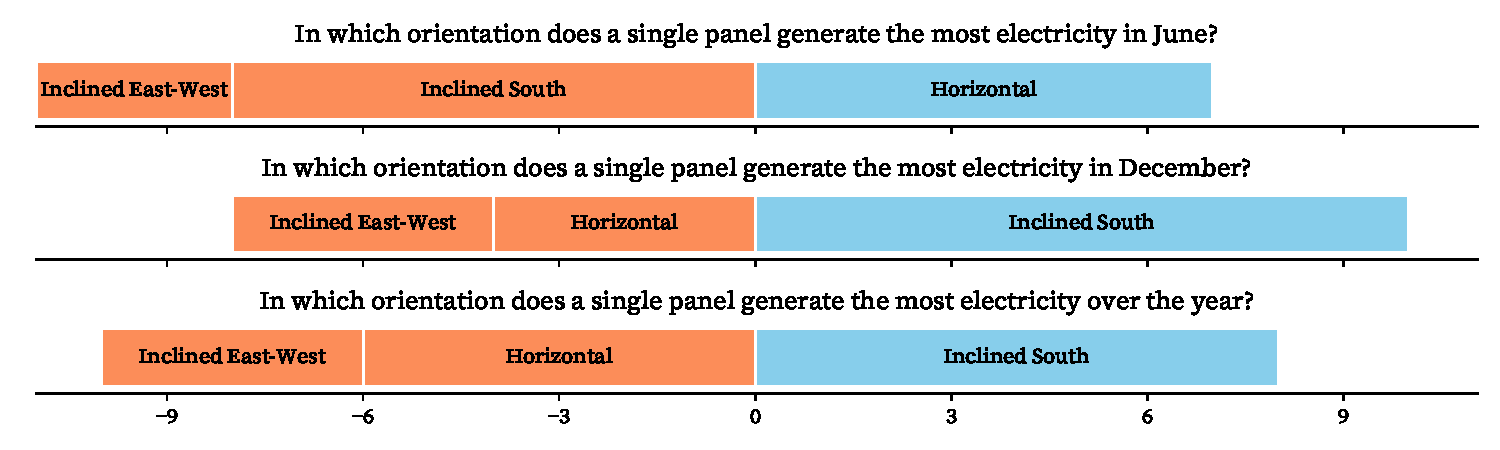
\includegraphics[width=\textwidth]{graphics/research-3.pdf}
    \caption{A stacked bar chart of participant responses on optimal panel orientation in different settings.}
    \label{fig:research-3}
\end{figure}

To test this hypothesis, participants' responses to specific knowledge-based questions were analyzed after interacting with the VR simulation. These questions were designed to assess understanding of the orientation of PV panels for maximum electricity production in June, December, and over the year. Correct answers were predetermined based on the simulation data.
% add link to figure
The Chi-square test is chosen here because of its direct applicability to categorical data. It's ideal for comparing the observed distribution of responses with what we would expect by chance, assuming that the VR simulation has no effect on comprehension and no prior knowledge is present. Because each participant's response is independent and the test is effective even with smaller sample sizes, it's a  suitable method for assessing the educational impact of the VR simulation. It shows how likely it is that the observed data would occur under the null hypothesis.

\textbf{June Orientation}
Out of 18 responses, only 7 were correct (38.9\%). The statistical tests support the null hypothesis (Chi-square: 2.333, P-value: 0.311), suggesting that the VR simulation did not significantly aid understanding of this concept.

\textbf{December Orientation}
With 10 out of 18 correct answers (55.6\%), the first signs were promising. However, the Chi-square test confirmed the null hypothesis (Chi-square: 4.000, P-value: 0.135), indicating a random distribution of answers.

\textbf{Annual Orientation}
The VR simulation seemed to have a modest effect, with 8 correct answers out of 18 (44.4\%). However, statistical analysis showed no significant increase in correct answers (Chi-square: 1.333, P-value: 0.513).

%\textbf{Summary}
While the analysis did not provide statistical evidence to reject the null hypothesis for Hypothesis 4, it did reveal a noticeable, though not substantial, level of factual knowledge among the participants. This suggests that while the VR simulation may have led to some understanding of PV panel orientation, the knowledge gained was not pronounced.

\chapter{Discussion}
The aim of this research was to investigate the effectiveness of VR in improving comprehension and engagement with photovoltaic systems, as part of wider environmental education initiatives. This chapter evaluates the extent to which these objectives were achieved, discussing the implications of the findings within the context of VR as a transformative educational tool.



It stands to reason that if participants were given specific tasks or instructions on what aspects to observe within the VR simulation, their performance and subsequent understanding may have improved. A more guided experience could potentially lead to better internalization of the concepts presented. It might also help participants to apply and observe these ideas more successfully during the interactive experience if a theoretical basis on orientation, the effects of angles and air mass was provided prior to the VR simulation. Such initial instruction could enhance their ability to recognise and understand the finer details of PV panel optimisation, leading to more thoughtful and informed observation. This hybrid method of combining immersive VR technology with theory has great potential for future educational projects aimed at improving students' understanding of renewable energy technologies and their real-world applications.

To improve the statistical validity of future research, the test design should be adapted to allow a comparison of participants' knowledge before and after the VR experience. The inability of the existing design to properly relate current knowledge to the VR simulation indicates a need for methodological improvements.

\section{Understanding Photovoltaic Systems through VR}
The user studies revealed significant improvements in the understanding of photovoltaic systems through the \textit{SolarPowerVR} application compared to the original \textit{KaisergasseVR}. Users reported high levels of engagement and a clearer understanding of photovoltaic mechanics, facilitated by the immersive and interactive nature of the VR environment.

\section{Overcoming Technical Challenges}
The development of the VR applications has been marked by significant technical hurdles, in particular the performance issues posed by the detailed and dynamic virtual representation of the Linz cityscape. The innovative solutions employed, including the use of the Cesium environment and the optimization of dynamic shadows, illustrate the critical importance of technical expertise in creating immersive and effective VR experiences. Introducing an in-game tutorial and refining the controls based on user feedback are key to improving the usability and educational impact of the VR application.

\section{Educational Impact and User Experience}
The migration from the \textit{KaisergasseVR} application to the \textit{SolarPowerVR} application demonstrated the crucial role of user experience design in educational VR applications. Simplifying interaction mechanisms and stabilising performance to achieve a consistently high frame rate contributed greatly to a more accessible and engaging learning environment. The detailed user feedback from the initial user study was instrumental in identifying and addressing shortcomings, resulting in the superior performance and educational effectiveness of \textit{SolarPowerVR}.

\section{Statistical Findings and Study Design}
While the statistical analysis provided insights into the learning outcomes associated with the VR applications, it also highlighted the limitations of the study design in conclusively determining the effectiveness of VR in improving understanding of renewable energy systems. The lack of significant findings regarding panel orientation post-experience suggests the need for a more robust research framework and a more guided approach within the VR application to ensure comprehensive learning.

\section{Future directions and considerations}
The exploration of photovoltaic systems in VR represents a promising avenue for environmental education. However, realizing its full potential requires addressing the challenges of accessibility, expanding the scope of the application to include additional renewable energy sources, and continuous refinement based on user feedback. Future research should aim to consolidate the study design to provide more conclusive evidence of the educational benefits of VR in this area.

\section{Reflections on personal development}
Developing the VR application and conducting the user studies has been a profound learning experience. The challenges faced and solutions found not only contribute to the field of educational technology, but also represent significant personal and professional development. This project has reinforced the importance of a focused, user-centered approach to technology development and the potential of VR as a transformative tool in environmental education and advocacy.

\chapter{Conclusion and future work}
This chapter evaluates the extent to which the stated objectives were achieved, identifies the limitations encountered during the research, and suggests future directions based on the empirical data and theoretical insights gained throughout the study.

The study demonstrated the potential of immersive technology in environmental education through the development and initial deployment of a VR application designed to demonstrate the operation and benefits of solar PV systems. User feedback highlighted the need for well-organized instruction within the VR environment to ensure a focused and educational experience. The lack of structured training and defined activities led to instances of user confusion, highlighting the importance of guided learning pathways in educational VR applications.

\section{Future Developments}
\begin{itemize}
    \item A tutorial is necessary to orient users within the VR environment. It should explain controls, simulation functions, and data interpretation methods. Subsequent activities should be designed to help users focus on learning objectives, such as assessing power output variances across different situations.
    \item Incorporating the LXR - Light Detection plugin can enhance the simulation's realism in light interaction, which is crucial for accurately representing PV shading behavior. Collaborating with PV installation specialists and using real-world price data can improve the simulation's portrayal of economic elements of PV systems.
    \item Future studies should use a strict methodological framework, including pre- and post-experience evaluations or control groups, to objectively quantify the influence of VR applications on users' understanding and attitudes towards PV systems.
    \item To promote user autonomy, VR applications should be self-explanatory. Expanding language support would improve accessibility, cater to a worldwide audience, and provide a broader educational effect.
    \item The exploration of industry sponsorship should also be considered. The first assistance of Linz City serves as a platform for further application development. To ensure widespread adoption and impact, it is crucial to identify industrial sponsors and integrate the VR application into educational contexts.
    \item Additionally, improving context awareness is necessary for the AI assistant to provide real-time, relevant instruction and act as an active learning facilitator in VR.
\end{itemize}

The creation of this VR application has been challenging and rewarding. The feedback and ideas gathered can pave the way for significant improvements that promise to make the application more entertaining, educational, and a catalyst for increased public interest in renewable energy solutions. Looking ahead, we are inspired by the potential of VR technology to improve environmental education and are determined to continue this fascinating mission.

\backmatter

% Use an optional list of figures.
\listoffigures % Starred version, i.e., \listoffigures*, removes the toc entry.

% Use an optional list of tables.
% \cleardoublepage % Start list of tables on the next empty right hand page.
% \listoftables % Starred version, i.e., \listoftables*, removes the toc entry.

% Use an optional list of alogrithms.
% \listofalgorithms
% \addcontentsline{toc}{chapter}{List of Algorithms}

% Add an index.
\printindex

% Add a glossary.
\printglossaries

% Add a bibliography.
\bibliographystyle{alpha}
% \bibliographystyle{plain}
\bibliography{main}

\end{document}
